%% Tudor Berariu, Alexandru Sorici
%% Noiembrie 2012

%%%%%%%%%%%%%%%%%%%%%%
%% Slide 0: Reaminitrea problemei pe care o rezolvăm

\begin{frame}
  \frametitle{Algoritmul Forward-Backward}
  \begin{block}{Problema Evaluării}
    Date fiind un model $\lambda = (A, B, \Pi)$ și o secvență de
    observații $O = [o_1 o_2 \ldots o_T]$, care este probabilitatea ca
    secvența de observații să fi fost produsă de acel model?
    \begin{equation}
      \label{eq:pb-evaluarii}
      P(O \vert \lambda) = ?
    \end{equation}
  \end{block}
  \pause
  \begin{block}{Rezolvare}
    $P(O \vert \lambda)$ se calculează \emph{eficient} cu algoritmul
    \alert{Forward - Backward}.\\\vspace*{1em}%
    Calculul se face cu ajutorul unor variabile auxiliare $\alpha$ și $\beta$.
  \end{block}
\end{frame}

%%%%%%%%%%%%%%%%%%%%%%
%% Slide 1: Motivația variabilelor alpha
\begin{frame}
  \frametitle{Variabilele $\alpha$ - Motivație}
  \begin{itemize}
  \item Calcul conform legii probabilităților totale:
    \begin{equation}
      \begin{split}
        P(O \vert \lambda) = \displaystyle\sum_{all\;Q} P(O, Q \vert
        \lambda) & = \displaystyle\sum_{all\;Q} P(O,\vert Q, \lambda)
        \cdot P(Q, \lambda) \\
        & = \displaystyle\sum_{\text{all}\;Q} \Big( \pi_{q_1} \cdot
        b_{q_1}(o_1) \cdot \displaystyle\prod_{t=2}^{T} b_{q_t}(o_t)
        a_{q_{t-1},q_t} \Big)
      \end{split}
      \tag{\ref{eq1}}
    \end{equation}
  \item Pentru secvențele de stări care încep cu o secvență comună
    $[q_1 q_2 \ldots q_Z]$, următorii factori sunt comuni:
    \begin{equation*}
      \pi_{q_1} \cdot
      b_{q_1}(o_1) \cdot \displaystyle\prod_{z=2}^{Z} b_{q_z}(o_z)
      a_{q_{z-1},q_z}
    \end{equation*}
    \begin{itemize}
    \item Calculul de $(T-Z)^N$ ori ar fi redundant!
    \end{itemize}

  \end{itemize}
\end{frame}


%%%%%%%%%%%%%%%%%%%%%%
%% Slide 2: Definiția variabilelor alpha
\begin{frame}
  \frametitle{Variabilele $\alpha$ - Definiție}
  \begin{block}{}
    Definim variabilele $\alpha$ astfel:
    \begin{equation}
      \label{eq:alpha}
      \begin{split}
        \alpha_{t,i}=P(o_1,o_2,\ldots,o_t, q_t = s_i \vert \lambda) \\
        \scriptstyle{1 \le t \le T, 1 \le i \le N}
      \end{split}
    \end{equation}
    (probabiliatea de a fi observat primele $t$ valori observate
    ajungând la momentul $t$ în starea $s_i$, dați fiind parametrii
    $\lambda$)
  \end{block}%  
  \pause%  
  \begin{block}{}
    Relația dintre $P(O \vert \lambda)$ și variabilele $\alpha$ este:
    \begin{equation}
      \label{eq:eq1toalpha}
      P(O \vert \lambda) = \displaystyle\sum_{i=1}^{N}\alpha_{T,i}
    \end{equation}
    (conform legii probabilităților totale)
  \end{block}%
\end{frame}

%%%%%%%%%%%%%%%%%%%%%%
%% Slide 3: Calculul variabilelor alpha
\begin{frame}
  \frametitle{Calculul variabilelor $\alpha$}
  \begin{columns}
    \column{0.38\textwidth}
    
\includegraphics[width=\textwidth]{graphics/forward-backward/general/forward.pdf}
    \column{0.62\textwidth}
    \begin{itemize}
    \item Inițializare ($t = 1$)%
      \begin{equation*}
        \alpha_{1,i}=\pi_ib_i(o_1), \quad 1 \le i \le N
      \end{equation*}\pause%
    \item Inducție ($t>1$)%
      \begin{equation*}
        \label{eq:alpha_induct}
        \alpha_{t+1,j}=\Big[
        \displaystyle\sum_{i=1}^{N}\alpha_{t,j}a_{i,j}\Big]
        b_{j}(o_{t+1}), \quad \substack{1 \le t \le T-1\\1\le j \le N}
      \end{equation*}\pause%
    \item Probabilitatea secvenței observate:
      \begin{equation*}
        \label{eq:alpha_term}
        P(O \vert \lambda) =
        \displaystyle\sum_{i=1}^{N}\alpha_{T,i}
      \end{equation*}
    \end{itemize}
  \end{columns}
\end{frame}

%%%%%%%%%%%%%%%%%%%%%%
%% Slide 4: Motivația variabilelor beta
\begin{frame}
  \frametitle{Variabilele $\beta$ - Definiție}
  \begin{block}{}
    Definim variabilele $\beta$ astfel:
    \begin{equation}
      \label{eq:beta}
      \beta_{t,i}=P(o_{t+1} o_{t+2} \cdots o_{T} \vert q_t = s_i,
      \lambda)
    \end{equation}

    (probabiliatea de a fi observate valorile secvenței de la $t+1$ la
    $T$, condiționată de aflarea la momentul $t$ în starea $s_i$ și de
    parametrii $\lambda$)
  \end{block}%
  \pause%  
  \begin{block}{}
    Relația dintre $P(O \vert \lambda)$ și variabilele $\beta$ este:
    \begin{equation}
      \label{eq:eq1toalpha}
      P(O \vert \lambda) = \displaystyle\sum_{i=1}^{N}\beta_{1,i}
    \end{equation}
    (conform legii probabilităților totale)
  \end{block}%
\end{frame}

%%%%%%%%%%%%%%%%%%%%%%
%% Slide 5: Calculul variabilelor beta
\begin{frame}
  \frametitle{Calculul Variabilelor $\beta$}
  \begin{columns}[B]
    \column{0.55\textwidth}
    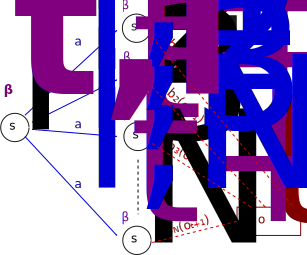
\includegraphics[width=\textwidth]{graphics/forward-backward/general/backward.pdf}
    \column{0.4\textwidth}
    \begin{itemize}
    \item Inițializare ($t=T$)
      \begin{equation}
        \beta_{T,i}=1,\quad 1 \le i \le N
        \label{eq:beta-init}
      \end{equation}
    \end{itemize}
  \end{columns}
  \begin{itemize}
  \item Pas de inducție ($t < T$) \\
    $\beta_{t,i}=\displaystyle\sum_{j=1}^{N}a_{i,j}b_j(o_{t+1})\beta_{t+1,j},
    \quad t = T-1, T-2, \ldots , 1, 1 \le i \le N$
  \end{itemize}
\end{frame}

%%%%%%%%%%%%%%%%%%%%%%
%% Slide 6: Probleme numerice
\begin{frame}
  \frametitle{Probleme numerice}
  \begin{itemize}
  \item să revedem definiția $P(O \vert \lambda)$:
    \begin{equation*}
      P(O \vert \lambda) = \displaystyle\sum_{\text{all}\;Q} \Big(
      \pi_{q_1} \cdot b_{q_1}(o_1) \cdot
      \displaystyle\prod_{t=2}^{T} b_{q_t}(o_t) a_{q_{t-1},q_t}
      \Big)
    \end{equation*}
    \pause
  \item toți cei 2$T$ factori ai unui produs sunt subunitari
  \item pentru secvențe mari, produsele se apropie mult de zero
  \item se depășește precizia disponibilă pentru reprezentare
  \item trebuie introdus un mecanism de \alert{scalare}
  \end{itemize}
\end{frame}


%%%%%%%%%%%%%%%%%%%%%%
%% Slide 7: Algoritm cu scalare
\begin{frame}
  \frametitle{Algoritmul Forward-Backward cu scalare}
  \begin{itemize}
  \item $\hat{\alpha}_{t,i}$ - variabilele $\alpha$ scalate
  \item $\hat{\beta}_{t,i}$ - variabilele $\beta$ scalate
    \vspace*{1em}
  \item $C_t$ - coeficienții de scalare \vspace*{1em}
  \item Variabilele $\alpha$ scalate
    \begin{equation}
      \label{eq:scaled-alpha}
      \hat{\alpha}_{t,i} = C_t \cdot \alpha_{t,i}
    \end{equation}
  \item Variabilele $\beta$ scalate:
    \begin{equation}
      \label{eq:scaled-beta}
      \hat{\beta}_{t,j} = C_t \cdot \beta_{t,j}
    \end{equation}
    (notațiile sunt adoptate din literatură) 
  \end{itemize}
\end{frame}

%%%%%%%%%%%%%%%%%%%%%%
%% Slide 8: Calcul alfa scalate
\begin{frame}
  \frametitle{Calculul variabilelor $\alpha$ scalate}
  \begin{columns}%
    \column{0.3\textwidth}%
    \begin{itemize}
    \item Inițializare ($t = 1$)\\\vspace*{1em}$1 \le i \le N$
    \end{itemize}%
    \column{0.7\textwidth}%
    \begin{align}%
      \ddot{\alpha}_{1,i} = \alpha_{1,i}\\
      c_1 = \frac{1}{\displaystyle\sum_{i=1}^{N}
        \ddot{\alpha}_{1,i}} \\
      \hat{\alpha}_{1,i} = c_1 \cdot \ddot{\alpha}_{1,i}
    \end{align}%
  \end{columns}%
  \vspace*{.5em} \pause \horiline
  \begin{columns}
    \column{0.3\textwidth}
    \begin{itemize}
    \item Pas de inducție ($t > 1$)\\\vspace*{1em}$1 \le j \le N$
    \end{itemize}%
    \column{0.7\textwidth}%
    \begin{align}%
      \ddot{\alpha}_{t+1,j} = \Big[
      \displaystyle\sum_{i=1}^{N}\hat{\alpha}_{t,i}a_{i,j}\Big]
      b_{j}(o_{t+1}) \\
      c_{t+1} = \dfrac{1}{\displaystyle\sum_{j=1}^{N}
        \ddot{\alpha}_{t+1,j}} \\
      \hat{\alpha}_{t+1,j} = c_{t+1} \cdot \ddot{\alpha}_{t+1,j}
    \end{align}%
  \end{columns}%
\end{frame}

%%%%%%%%%%%%%%%%%%%%%%
%% Slide 9: Coeficienți
\begin{frame}[t]
  \frametitle{Coeficienții de scalare}
  Vom nota: $C_t = c_1 \cdot c_2 \cdot \ldots \cdot c_t$\\\vspace*{1em}%
  \textbf{Ipoteza}: $\hat{\alpha}_{t,i} = C_t\alpha_{t,i}$\\\vspace*{1em}%
  \only<2-3>{%
    Demonstrație prin inducție:
    \begin{itemize}
    \item ($t=1$):
      \begin{equation*}
        \hat{\alpha}_{1,i} = c_1 \cdot \ddot{\alpha}_{1,i} = c_1 \cdot \alpha_{1,i}
      \end{equation*}%
      \visible<3>{%
      \item ($t>1$): Presupunem adevărat: $\hat{\alpha}_{t,i} = C_{t}\alpha_{t,i}$%
        \begin{align*}%
          \ddot{\alpha}_{t+1,j} & = \Big[
          \displaystyle\sum_{i=1}^{N}\hat{\alpha}_{t,i}a_{i,j}\Big]
          b_{j}(o_{t+1}) = \Big[
          \displaystyle\sum_{i=1}^{N}C_{t}\alpha_{t,i}a_{i,j}\Big]
          b_{j}(o_{t+1}) = C_{t} \alpha_{t+1,j} \\
          \hat{\alpha}_{t+1,j} & = c_{t+1} \cdot \ddot{\alpha}_{t+1,j} = c_{t+1} \cdot C_{t} \cdot\alpha_{t+1,j} = C_{t+1}\cdot\alpha_{t+1,j}
        \end{align*}%
      }%
    \end{itemize}%
  }%
  \only<4-7>{%
    Atunci:  $\mathbf{P(O \vert \lambda)} = \displaystyle\sum_{i=1}^{N}\alpha_{T,i} = 
    C^{-1}_T \cdot \displaystyle\sum_{i=1}^{N}\hat{\alpha}_{T,i} = C^{-1}_T = \mathbf{\displaystyle\prod_{t=1}^{T}c^{-1}_t}$\\\vspace*{1em}%
    \only<5-7>{%
      Calculăm $P(O \vert \lambda)$?
    }%
    \only<6-7>{%
      \textbf{\alert{NU}}\\
    }%
    \vspace*{1em}%
    \visible<7>{%
      Calculăm:
      \begin{equation}
        \label{eq:logP}
        log(P(O \vert \lambda)) = log(\displaystyle\prod_{t=1}^{T}c^{-1}_t) = \displaystyle\sum_{t=1}^{T}log(c_t^{-1}) = -\displaystyle\sum_{t=1}^{T}log(c_t)
      \end{equation}%
    }%
  }%
\end{frame}

%%%%%%%%%%%%%%%%%%%%%%
%% Slide 8: Calcul beta scalate
\begin{frame}
  \frametitle{Calculul variabilelor $\beta$ scalate}
  \begin{columns}%
    \column{0.3\textwidth}%
    \begin{itemize}
    \item Inițializare ($t = T$)\\\vspace*{1em}$1 \le i \le N$
    \end{itemize}%
    \column{0.7\textwidth}%
    \begin{align}%
      \ddot{\beta}_{T,i} = \beta_{T,i} = 1\\
      \hat{\beta}_{T,i} = c_T \cdot \ddot{\beta}_{T,i}
    \end{align}%
  \end{columns}%
  \vspace*{.5em} \pause \horiline
  \begin{columns}
    \column{0.3\textwidth}
    \begin{itemize}
    \item Pas de inducție ($t < T$)\\\vspace*{1em}$1 \le i \le N$
    \end{itemize}%
    \column{0.7\textwidth}%
    \begin{align}%
      \ddot{\beta}_{t,i} = \displaystyle\sum_{j=1}^{N}a_{i,j}b_{j}(o_{t+1})\hat{\beta}_{t+1,i}\\
      \hat{\beta}_{t,i} = c_{t} \cdot \ddot{\beta}_{t,i}
    \end{align}%
  \end{columns}%
  \begin{itemize}
  \item Se demonstrează: $\hat{\beta}_{t,i}=c_t \cdot c_{t+1} \cdot \ldots \cdot c_T \cdot \beta_{t,i}$
  \end{itemize}
\end{frame}

\begin{frame}
  \frametitle{Exemplu de aplicație}
  \begin{itemize}
    \item Să reluăm exemplul de mai devreme cu robotul.
    \item Robotul acționează diferit în fața a 2 tipuri de personalitate:
      \begin{itemize}
      \item \emph{jovialul}
      \item \emph{morocănosul}.
      \end{itemize}
    \item Pentru fiecare există un set de parametri:
      \begin{itemize}
      \item $\lambda^{1}=(A^{1},B^{1},\Pi^{1})$
      \item $\lambda^{2}=(A^{2},B^{2},\Pi^{2})$
      \end{itemize}
    \item Robotul recunoaște următoarele gesturi:\\
      \alert{(zâmbet $\vert$ rânjet)} $\longrightarrow$ \alert{(zâmbet $\vert$ rânjet)} $\longrightarrow$ \alert{încruntare}%
      \vspace*{1em}
    \item \textbf{Întrebare:} Cărei personalități este mai probabil să-i aparțină cel monitorizat?
  \end{itemize}
\end{frame}

\begin{frame}%
  \frametitle{Jovialul}%
  \begin{columns}[T]%
    \column{0.58\textwidth}%
    \only<1>{\framebox{\includegraphics[width=\textwidth]{graphics/forward-backward/guys/good-guy-q.pdf}}}%
    \only<2>{\framebox{\includegraphics[width=\textwidth]{graphics/forward-backward/guys/good-guy-r.pdf}}}%
    \only<3>{\framebox{\includegraphics[width=\textwidth]{graphics/forward-backward/guys/good-guy-s.pdf}}}%
    \only<4>{\framebox{\includegraphics[width=\textwidth]{graphics/forward-backward/guys/good-guy-t.pdf}}}%
    \only<5>{\framebox{\includegraphics[width=\textwidth]{graphics/forward-backward/guys/good-guy-u.pdf}}}%
    \only<6>{\framebox{\includegraphics[width=\textwidth]{graphics/forward-backward/guys/good-guy-v.pdf}}}%
    \only<7>{\framebox{\includegraphics[width=\textwidth]{graphics/forward-backward/guys/good-guy-w.pdf}}}%
    \only<8>{\framebox{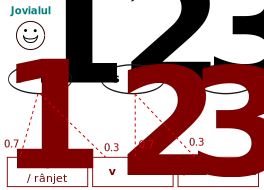
\includegraphics[width=\textwidth]{graphics/forward-backward/guys/good-guy-x.pdf}}}%
    \only<9>{\framebox{\includegraphics[width=\textwidth]{graphics/forward-backward/guys/good-guy-y.pdf}}}%
    \only<10>{\framebox{\includegraphics[width=\textwidth]{graphics/forward-backward/guys/good-guy-z.pdf}}}%
    \column{0.41\textwidth}%
    $\lambda^{1}=(A^{1},B^{1},\Pi^{1})$\\\vspace*{1em}%
    $A^{1} = \bordermatrix{~ & s_1 &
      s_2 & s_3 \cr s_1 &     \visible<2->{0.8} & \visible<2->{0.1} & \visible<2->{0.1} \cr s_2 &
      \visible<3->{0.25} & \visible<3->{0.25} & \visible<3->{0.5}
      \cr s_3 & \visible<4->{0.8} & \visible<4->{0.2} &
      \visible<4->{0} \cr}$\\\vspace*{1em}%
    $\Pi^{1} = \bordermatrix{ ~ & s_1 & s_2 & s_3 \cr ~ 
      & \visible<5->{0.7} & \visible<5->{0.2} & \visible<5->{0.1} \cr}$\\\vspace*{1em}%
    $B^{1} = \bordermatrix{~ & v_1 &
      v_2 & v_3 \cr s_1 & \visible<7->{0.7} & \visible<7->{0.3} & \visible<7->{0} \cr s_2 &
          \visible<8->{0} & \visible<8->{0.7} & \visible<8->{0.3}
          \cr s_3 & \visible<9->{0.6} & \visible<9->{0} &
          \visible<9->{0.4} \cr}$
  \end{columns}%
\end{frame}%

\begin{frame}%
  \frametitle{Morocănosul}%
  \begin{columns}[T]%
    \column{0.58\textwidth}%
    \only<1>{\framebox{\includegraphics[width=\textwidth]{graphics/forward-backward/guys/surly-guy-q.pdf}}}%
    \only<2>{\framebox{\includegraphics[width=\textwidth]{graphics/forward-backward/guys/surly-guy-r.pdf}}}%
    \only<3>{\framebox{\includegraphics[width=\textwidth]{graphics/forward-backward/guys/surly-guy-s.pdf}}}%
    \only<4>{\framebox{\includegraphics[width=\textwidth]{graphics/forward-backward/guys/surly-guy-t.pdf}}}%
    \only<5>{\framebox{\includegraphics[width=\textwidth]{graphics/forward-backward/guys/surly-guy-u.pdf}}}%
    \only<6>{\framebox{\includegraphics[width=\textwidth]{graphics/forward-backward/guys/surly-guy-v.pdf}}}%
    \only<7>{\framebox{\includegraphics[width=\textwidth]{graphics/forward-backward/guys/surly-guy-w.pdf}}}%
    \only<8>{\framebox{\includegraphics[width=\textwidth]{graphics/forward-backward/guys/surly-guy-x.pdf}}}%
    \only<9>{\framebox{\includegraphics[width=\textwidth]{graphics/forward-backward/guys/surly-guy-y.pdf}}}%
    \only<10>{\framebox{\includegraphics[width=\textwidth]{graphics/forward-backward/guys/surly-guy-z.pdf}}}%
    \column{0.41\textwidth}%
    $\lambda^{2}=(A^{2},B^{2},\Pi^{2})$\\\vspace*{1em}%
    $A^{2} = \bordermatrix{~ & s_1 &
      s_2 & s_3 \cr s_1 &     \visible<2->{0.5} & \visible<2->{0.3} & \visible<2->{0.2} \cr s_2 &
      \visible<3->{0.1} & \visible<3->{0.6} & \visible<3->{0.3}
      \cr s_3 & \visible<4->{0.4} & \visible<4->{0.5} &
      \visible<4->{0.1} \cr}$\\\vspace*{1em}%
    $\Pi^{2} = \bordermatrix{ ~ & s_1 & s_2 & s_3 \cr ~ 
      & \visible<5->{0.3} & \visible<5->{0.5} & \visible<5->{0.2} \cr}$\\\vspace*{1em}%
    $B^{2} = \bordermatrix{~ & v_1 &
      v_2 & v_3 \cr s_1 & \visible<7->{0.4} & \visible<7->{0.5} & \visible<7->{0.1} \cr s_2 &
          \visible<8->{0} & \visible<8->{0.2} & \visible<8->{0.8}
          \cr s_3 & \visible<9->{0.6} & \visible<9->{0} &
          \visible<9->{0.4} \cr}$
  \end{columns}%
\end{frame}%

\begin{frame}
  \frametitle{Calculul variabilelor $\alpha$:}%
  \begin{columns}%
    \column{0.57\textwidth}
    \only<1>{\framebox{\includegraphics[width=\textwidth]{graphics/forward-backward/compute-alpha/compute-alpha-none.pdf}}}%
    \only<2>{\framebox{\includegraphics[width=\textwidth]{graphics/forward-backward/compute-alpha/compute-alpha-11.pdf}}}%
    \only<3>{\framebox{\includegraphics[width=\textwidth]{graphics/forward-backward/compute-alpha/compute-alpha-12.pdf}}}%
    \only<4>{\framebox{\includegraphics[width=\textwidth]{graphics/forward-backward/compute-alpha/compute-alpha-13.pdf}}}%
    \only<5-6>{\framebox{\includegraphics[width=\textwidth]{graphics/forward-backward/compute-alpha/compute-alpha-1.pdf}}}%
    \only<7>{\framebox{\includegraphics[width=\textwidth]{graphics/forward-backward/compute-alpha/compute-alpha-21.pdf}}}%
    \only<8>{\framebox{\includegraphics[width=\textwidth]{graphics/forward-backward/compute-alpha/compute-alpha-22.pdf}}}%
    \only<9>{\framebox{\includegraphics[width=\textwidth]{graphics/forward-backward/compute-alpha/compute-alpha-23.pdf}}}%
    \only<10-11>{\framebox{\includegraphics[width=\textwidth]{graphics/forward-backward/compute-alpha/compute-alpha-2.pdf}}}%
    \only<12>{\framebox{\includegraphics[width=\textwidth]{graphics/forward-backward/compute-alpha/compute-alpha-31.pdf}}}%
    \only<13>{\framebox{\includegraphics[width=\textwidth]{graphics/forward-backward/compute-alpha/compute-alpha-32.pdf}}}%
    \only<14>{\framebox{\includegraphics[width=\textwidth]{graphics/forward-backward/compute-alpha/compute-alpha-33.pdf}}}%
    \only<15-16>{\framebox{\includegraphics[width=\textwidth]{graphics/forward-backward/compute-alpha/compute-alpha-3.pdf}}}%
    \vspace*{2em}%
     \\$\hat{\alpha} = \begin{bmatrix}
       \scriptstyle \visible<6->{0.8909} & \scriptstyle \visible<6->{0} & \scriptstyle \visible<6->{0.1091} \\
       \scriptstyle \visible<11->{0.9128} & \scriptstyle \visible<11->{0} & \scriptstyle \visible<11->{0.0872} \\
       \scriptstyle \visible<16->{0} & \scriptstyle \visible<16->{0.4718} & \scriptstyle \visible<16->{0.5282}\end{bmatrix} \:
     c = \begin{bmatrix} 
      \scriptstyle \visible<5->{1.8182} \\ 
      \scriptstyle \visible<10->{1.63} \\ 
      \scriptstyle \visible<15->{14.4718}\end{bmatrix}$
    \vspace*{3em}%
    \column{0.43\textwidth}
    \only<2-6>{%
      \begin{align*}
        \scriptstyle \ddot{\alpha}_{1,1}=\pi_{1,1}\cdot b_1(v_1)=0.7\cdot 0.7 = 0.49 \\
        \visible<3->{%
          \scriptstyle \ddot{\alpha}_{1,2}=\pi_{1,2}\cdot b_2(v_1)=0.2\cdot 0 = 0 \\
        }
        \visible<4->{%
          \scriptstyle \ddot{\alpha}_{1,3}=\pi_{1,3}\cdot b_3(v_1)=0.1\cdot 0.6 = 0.6 \\
        }%
      \end{align*}%
      \visible<5->{%
        \vspace*{-4em}\horiline\vspace*{-.5em}%
        \begin{align*}
          \scriptstyle c_1 & \scriptstyle = \frac{1}{\ddot{\alpha}_{1,1} + \ddot{\alpha}_{1,2} +
            \ddot{\alpha}_{1,3}} \\\scriptstyle c_1 & \scriptstyle  = 1 / 0.54 \approx 1.8182
        \end{align*}%
        \visible<6->{%
          \vspace*{-2.5em}\horiline\vspace*{-.5em}%
          \begin{align*}
            \scriptstyle \hat{\alpha}_{1,1} & \scriptstyle = c_1 \cdot \ddot{\alpha}_{1,1} = 0.8909 \\
            \scriptstyle \hat{\alpha}_{1,2} & \scriptstyle = c_1 \cdot \ddot{\alpha}_{1,2} = 0\\
            \scriptstyle \hat{\alpha}_{1,3} & \scriptstyle = c_1 \cdot \ddot{\alpha}_{1,3} = 0.1091
          \end{align*}%
        }%
      }%
    }%
    \only<7-11>{%
      \begin{align*}%
        \scriptstyle \ddot{\alpha}_{2,1} & \scriptstyle =b_1(v_1)\sum\hat{\alpha}_{1,i}a_{i,1} \\
        & \scriptstyle = \ldots = 0.56 \\
        \visible<8->{%
          \scriptstyle \ddot{\alpha}_{2,2} & \scriptstyle =b_2(v_1) \sum \hat{\alpha}_{1,i}a_{i,2} = 0\\
        }%
        \visible<9->{%
          \scriptstyle \ddot{\alpha}_{2,3} & \scriptstyle =b_3(v_1) \sum \hat{\alpha}_{1,i}a_{i,3} = 0.0535
        }%
      \end{align*}%
      \visible<10->{%
        \vspace*{-2.5em}\horiline\vspace*{-.5em}%
        \begin{align*}
          \scriptstyle c_2 & \scriptstyle = \frac{1}{\ddot{\alpha}_{2,1} + \ddot{\alpha}_{2,2} + \ddot{\alpha}_{2,3}} \\\scriptstyle c_2 & \scriptstyle  = \frac{1}{0.484+0.0776+0} = 1.63
        \end{align*}%
        \visible<11->{%
          \vspace*{-2.5em}\horiline\vspace*{-.5em}%
          \begin{align*}
            \scriptstyle \hat{\alpha}_{2,1} & \scriptstyle = c_2 \cdot \ddot{\alpha}_{2,1} = 0.9128 \\
            \scriptstyle \hat{\alpha}_{2,2} & \scriptstyle =c_2 \cdot \ddot{\alpha}_{2,2} = 0 \\
            \scriptstyle \hat{\alpha}_{2,3} & \scriptstyle =c_2 \cdot \ddot{\alpha}_{2,3} = 0.0872
          \end{align*}%
        }%
      }%
    }%
    \only<12-16>{%
      \begin{align*}%
        \scriptstyle \ddot{\alpha}_{3,1} & \scriptstyle =b_1(v_3)\sum\hat{\alpha}_{2,i}a_{i,1} \\
        & \scriptstyle = \ldots = 0 \\
        \visible<13->{%
          \scriptstyle \ddot{\alpha}_{3,2} & \scriptstyle =b_2(v_3) \sum \hat{\alpha}_{2,i}a_{i,2} = 0.0326\\
        }%
        \visible<14->{%
          \scriptstyle \ddot{\alpha}_{3,3} & \scriptstyle =b_3(v_3) \sum \hat{\alpha}_{2,i}a_{i,3} = 0.0365
        }%
      \end{align*}%
      \visible<15->{%
        \vspace*{-2.5em}\horiline\vspace*{-.5em}%
        \begin{align*}
          \scriptstyle c_3 & \scriptstyle = \frac{1}{\ddot{\alpha}_{3,1} + \ddot{\alpha}_{3,2} + \ddot{\alpha}_{,3}} \\\scriptstyle c_3 & \scriptstyle  = \frac{1}{0.069} = 14.4718
        \end{align*}%
        \visible<16->{%
          \vspace*{-2.5em}\horiline\vspace*{-.5em}%
          \begin{align*}
            \scriptstyle \hat{\alpha}_{3,1} & \scriptstyle = c_3 \cdot \ddot{\alpha}_{3,1} = 0 \\
            \scriptstyle \hat{\alpha}_{3,2} & \scriptstyle =c_3 \cdot \ddot{\alpha}_{3,2} = 0.4718 \\
            \scriptstyle \hat{\alpha}_{3,3} & \scriptstyle =c_3 \cdot \ddot{\alpha}_{3,3} = 0.5282
          \end{align*}%
        }%
      }%
    }%
  \end{columns}%
\end{frame}

\begin{frame}
  \frametitle{Morocănos sau jovial?}
  \begin{itemize}
    \item $c = \begin{bmatrix} \scriptstyle 1.8182 & \scriptstyle 1.63 &  \scriptstyle 14.4718\end{bmatrix}$
    \item Probabilitatea ca secvența observată să fi fost generată de un \emph{jovial}:\\
      $\log(P(O\vert \lambda^{1}))=-\displaystyle\sum\log(c_i) = -3.7583$\\\vspace*{1em}\pause%
    \item Probabilitatea ca secvența observată să fi fost generată de un \emph{morocănos}:\\
      $\log(P(O\vert \lambda^{2}))=-3.6362$\\\vspace*{1em}%\pause
    \item $\log(P(O\vert \lambda^{2})) > \log(P(O\vert \lambda^{1}))$
    \item Este mai probabil să avem de-a face cu un...\pause\\\vspace*{.5em}%
      \begin{center}\includegraphics{graphics/forward-backward/guys/surly-face.pdf}\end{center}
    \end{itemize}
\end{frame}

\begin{frame}
  \frametitle{Calculul variabilelor $\beta$:}
    \begin{columns}%
    \column{0.6\textwidth}
    \only<1>{\framebox{\includegraphics[width=\textwidth]{graphics/forward-backward/compute-beta/compute-beta-none.pdf}}}%
    \only<2>{\framebox{\includegraphics[width=\textwidth]{graphics/forward-backward/compute-beta/compute-beta-31.pdf}}}%
    \only<3>{\framebox{\includegraphics[width=\textwidth]{graphics/forward-backward/compute-beta/compute-beta-32.pdf}}}%
    \only<4>{\framebox{\includegraphics[width=\textwidth]{graphics/forward-backward/compute-beta/compute-beta-33.pdf}}}%
    \only<5>{\framebox{\includegraphics[width=\textwidth]{graphics/forward-backward/compute-beta/compute-beta-21.pdf}}}%
    \only<6>{\framebox{\includegraphics[width=\textwidth]{graphics/forward-backward/compute-beta/compute-beta-22.pdf}}}%
    \only<7>{\framebox{\includegraphics[width=\textwidth]{graphics/forward-backward/compute-beta/compute-beta-23.pdf}}}%
    \only<8>{\framebox{\includegraphics[width=\textwidth]{graphics/forward-backward/compute-beta/compute-beta-11.pdf}}}%
    \only<9>{\framebox{\includegraphics[width=\textwidth]{graphics/forward-backward/compute-beta/compute-beta-12.pdf}}}%
    \only<10>{\framebox{\includegraphics[width=\textwidth]{graphics/forward-backward/compute-beta/compute-beta-13.pdf}}}%
  \end{columns}%
\end{frame}


\begin{frame}[fragile]
  \frametitle{Algoritmul Forward-Backward} \vspace*{-1.5em}
  \begin{columns}[T]
    \column{0.5\textwidth}
    \begin{algorithm}[H]
      \scriptsize
      \caption{Calculul variabilelor $\alpha$}
      \label{alg1}
      \algsetup{linenosize=\tiny} \algsetup{indent=2.25em}
      \begin{algorithmic}[2]
        \FOR{$i=1$ to $N$} \STATE $\ddot{\alpha}_{1,i} \leftarrow
        \pi_i \cdot b_i(o_1)$
        \ENDFOR
        \STATE $c_1 \leftarrow (\displaystyle\sum_{i=1}^{N}
        \ddot{\alpha}_{1,i})^{-1}$ \FOR{$i=1$ to $N$} \STATE
        $\hat{\alpha}_{1,i} \leftarrow c_1 \cdot \ddot{\alpha}_{1,i}$
        \ENDFOR
        \FOR{$t=1$ to $T-1$} \FOR{$j=1$ to $N$} \STATE
        $\ddot{\alpha}_{t+1,j} \leftarrow \Big[
        \displaystyle\sum_{i=1}^{N}\hat{\alpha}_{t,i}a_{i,j}\Big]
        b_{j}(o_{t+1})$
        \ENDFOR
        \STATE $c_{t+1} \leftarrow (\displaystyle\sum_{i=1}^{N}
        \ddot{\alpha}_{t+1,i})^{-1}$ \FOR{$i=1$ to $N$} \STATE
        $\hat{\alpha}_{t+1,i} \leftarrow c_{t+1} \cdot
        \ddot{\alpha}_{t+1,i}$
        \ENDFOR
        \ENDFOR
      \end{algorithmic}
    \end{algorithm}
    \column{0.5\textwidth}
    \begin{algorithm}[H]
      \scriptsize
      \caption{Calculul $P(O \vert \lambda)$}
      \label{alg2}
      \algsetup{linenosize=\tiny} \algsetup{indent=2em}
      \begin{algorithmic}[2]
        \STATE $logP \leftarrow -\displaystyle\sum_{t=1}^{T}\log c_t$
      \end{algorithmic}
    \end{algorithm}
    \vspace*{1em}
    \begin{algorithm}[H]
      \scriptsize
      \caption{Calculul variabilelor $\beta$}
      \label{alg3}
      \algsetup{linenosize=\tiny} \algsetup{indent=2em}
      \algsetup{linenosize=\tiny}
      \begin{algorithmic}[2]
        \FOR{$i=1$ to $N$} \STATE $\hat{\beta}_{T,i} \leftarrow c_T$
        \ENDFOR
        \FOR{$t=(T-1)$ to $1$} \FOR{$i=1$ to $N$} \STATE
        $\hat{\beta}_{t,i} \leftarrow \displaystyle\sum_{j=1}^{N}
        a_{i,j} b_{j}(o_{t+1}) \hat{\beta}_{t+1,j} \cdot c_t$
        \ENDFOR
        \ENDFOR
      \end{algorithmic}
    \end{algorithm}
  \end{columns}
\end{frame}

\begin{frame}
  \frametitle{A venit vremea să scriem cod}
  \begin{enumerate}
  \item Faceți o copie a fișierului \texttt{forward\_backward\_disc.m.stub} 
    și denumiți-o \texttt{forward\_backward\_disc.m} (eliminați sufixul \texttt{.stub}).
    \\Veți implementa funcția:\\
    \mcode{function [logP, Alpha, Beta, Scale] = forward_backward_disc(O,Pi, A, B)}
    \pause
  \item Completați cele trei secțiuni (calcul $Alpha$, $Beta$ și $logP$).%
    \vspace*{-.5em}
    \lstinputlisting{m-files/forward.m}
\item Folosiți \mcode{hmm_test} pentru a vă testa codul.
\end{enumerate}
\end{frame}
